\documentclass[a4paper,10.0pt,twoside]{npr}

\usepackage{multicol,graphicx,lastpage,footmisc,fancyhdr,paralist,
tabularx,array,booktabs,caption,multirow,upgreek,mathrsfs,gensymb,color}
\usepackage[fancyhdr,space,fntef,fontset=ubuntu]{ctex}
\usepackage{amssymb,bm,mathrsfs,bbm,amscd}
\usepackage{flushend,cuted}
\usepackage{refcount}
\usepackage{savesym}
\usepackage{textcomp}
\usepackage[tbtags]{amsmath}  %
\savesymbol{iint}
\usepackage{amstext} %数学宏包文本命令
\usepackage{balance} %版心底部对齐

\flushbottom      %版心底部对齐
\setcounter{section}{0}
\begin{document}
%\begin{CJK*}{GBK}{\song}{\wuhao}{\rm}

%___________________________________________________________________________________
\def\rd{{\rm d}}

\newcommand{\RM}{\ensuremath{\mathrm}}   %正体 既可用于文本模式也可用于数学模式
\newcommand{\dif}{\mathrm{d}}  %直立体d
\newcommand{\me}{\mathrm{e}}  %直立体e
\newcommand{\mi}{\mathrm{i}}  %直立体i
\newcommand{\mj}{\mathrm{j}}  %直立体j
\newcommand{\afrac}[2]{\dfrac{\,#1\,}{\,#2\,}}  %略长分数线
\newcommand{\nn}{\nonumber}  %公式无编号
\newcommand{\nt}{\noindent}
\newcommand{\OO}{~\text{。}}
\newcommand{\PP}{~\text{,}}
\newcommand{\OP}{~\text{;}}
\newcommand{\LT}{\left}
\newcommand{\RT}{\right}

%___________________________________________________________________________________

\balance
\fancypagestyle{myfoot}
{%
\fancyhf{}
\fancyhead[c]{\wuhao\song 高~等~核~物~理~实~验}
\renewcommand{\headrule}{\vskip 2pt
\hrule height0.4pt width\headwidth \vskip1pt
\hrule height0.4pt width\headwidth \vskip-1.8pt}
}%
\thispagestyle{myfoot}

%%%%%%%%%%%%%%%%%%%%%%%%%%%%%%%%%%%%%%%%%%%%%%%%%%%%%
%    奇偶页眉
%%%%%%%%%%%%%%%%%%%%%%%%%%%%%%%%%%%%%%%%%%%%%%%%%%%%%
\pagestyle{fancy}
\fancyhead{}
\fancyhead[ce]{\xiaowu\song \hspace{0.5em}高~等~核~物~理~实~验}
%\fancyhead[ro,le]{\xiaowuhao \hspace{0.5em}\textbf{\textperiodcentered}\;\thepage\;\textbf{\textperiodcentered}\hspace{0.5em}}
%\fancyhead[ce]{\xiaowu\song 粒~子~物~理~与~原~子~核~物~理~专~题~实~验}
%\fancyhead[re]{\xiaowu\song \hspace{0.5em}第\;31\;卷\hspace{0.5em}}
\fancyfoot[ce,co]{}
\renewcommand{\headrule}{\vskip 2pt
\hrule height0.4pt width\headwidth}


\setcounter{page}{001}%
\fancyhead[co]{\xiaowuhao\song  乔颢:逆矩阵法解析$\gamma$能谱}    %奇页页眉
\begin{center}
\title{%
\xiaoerhao \bf  %章标题为两行时改为 \exiaoer
逆矩阵法解析$\gamma$能谱\\[-5mm]}
\maketitle
\large \fs
乔颢$^{^1}$\\[2mm]

\xiaowu \song
1. 北京大学物理学院,海淀区 北京 100871;\\[4mm]

 
\footnotetext[0]{{\bf 作者简介:}~~\begin{minipage}[t][4.2mm]{149mm}\song
乔颢,E-mail: i@catofes.com
\end{minipage} }
%\footnotetext[0]{{\bf 通信作者:}\song ~~E-mail: xxx@xxx.xxx }%通信作者为第一作者时不要此项

\parbox{158mm} {
\zywu{\bf 摘要:}~~\fs
本次实验通过求解逆矩阵的方法解析混合样品中各核素的活度,实验中混合样品由三种已知
的核素组成:$^{137}$Cs、$^{60}$Co、$^{54}$Mn, 其活度分别为:$1.0210\times 10^{5}$Bq、$5.3673\times 10^{4}$Bq、$4.7943\times 10^{4}$Bq。\\

{\bf 关键词:}~~\fs 逆矩阵,放射源活度,特征道域}\\
\end{center}
%%%%6.正文
\vspace{5mm}
%%%%6.正文
\setcounter{section}{0}
\begin{multicols}{2}
%----------------
%____________________________________________________________________________
%%%%以上请不要改动%%%%%%%%%%%%%%%%%%%%%%%%%%%%%%%%%%%%%%%%%%%%

\section{引言}    %1
\vspace*{-1mm}
\song\wuhao
对于已知核素的混合样品中核素进行活度分析,可以通过测量和分析$\gamma$射线的能谱来得到。

本次时实验中使用的$\gamma$探测器是NaI(TL)闪烁体探测器。在分析混合样品的时候,因为多种的能量射线混合,各个全能峰之间相互重迭,更不易区分,这就需要对混合样品的能谱进
行解析,从而确定组成混合样品中各核素的活度。

使用逆矩阵解谱需要满足一下的条件:

\begin{enumerate}
\item 混合样品中的核素都是已知的,因此可以测量相应样品的标准谱。
\item 测量标准谱和混合样品谱时,测量的条件不变。
\item 各个单一核素放射性线性叠加的情况下,探测系统的脉冲幅度不随计数率改变。
\item 混合样品中的各核素具有各自的$\gamma$能谱,并能够选出表征各自能量的特征峰。
\end{enumerate}

\section{实验原理}
本次实验中的混合样品有三种核素组成:$^{60}$Co、$^{137}$Cs、$^{54}$Mn,它们的放射性活度为$x_{i}$是未知量。在混合样品$\gamma$射线谱中,对四种核素选择一个既能够表征各自能量的特征峰,又能区别于其他核素的全能峰,称为该核素的特征全能峰。在这个全能峰上选择一个对称于最高计数处的道域称为特征道域。一般道域序数用i表示(i=1,2,,,)。测量每个核素的标准谱时,不仅要测量它在本身的特征道域中的计数,而且要测出它在其它特征道域中的计数,由此来确定各种核素对各个道域技术的贡献,这个贡献用响应系数$a_{ij}$来表示。$a_{ij}$为谱仪i道域对第j种核素的响应系数。其数值定义为:\\
\begin{equation}
a_{ij}=\frac{\text{第j种核素标准谱在i道阈上的计数率}}{\text{第j种核素标准样品的衰变率}};
\end{equation}
此响应系数取决于第j种成分各$\gamma$射线的相对强度和谱仪的测量条件。其意义是第j种核素的衰变率在i道域上所引起的计数率。混合样品在任意一个道域中的计数率可以分解为各个核素分别在该道域中引起的计数率之和,即:
\begin{equation}
\sum_{j=1}^{3}a_{ij}x_{i}=m_{i}    ~~~~(i=1,2,3);
\end{equation}
此方程可以用逆矩阵法求解,将方程组写成矩阵形式:
\begin{equation}
A \cdot X=M
\end{equation}
A为$a_{ij}$所组成的矩阵,称为谱仪对标准样品的响应矩阵,X为未知量$x_{i}$组成的列矩阵,M为各道域计数率组成的列矩阵。如果求出A的逆矩阵,则可得:
\begin{equation}
X=A^{-1}M
\end{equation}
即:
\begin{equation}
x_{i}=\sum_{i=1}^{3}a_{ji}^{-1}m_{i}
\end{equation}
因此由实验测定A,求出逆矩阵,再把测得的各特征道域上的计数率$m_{i}$代入,即可算出该混合样品中各核素的活度$x_{i}$。

逆矩阵法对某核素的分析精度,取决于在它的特征道阈中该核素计数在样品总计数中所占的份额,份额越大,分析精度越高,因此该核素的特征道阈应尽量选在该核素计数相对强度较大,而其他核素计数贡献少的全能峰上。被测样品在各特征道域上的计数和谱仪本底都会有统计涨落,并且通过逆矩阵计算互相传递。假如标准谱的测量精度足够高,使响应系数的误差可以忽略。根据误差理论可以推算出第j成分含量$x_{i}$的标准误差$\sigma _{\lambda }$为:
\begin{equation}
\sigma _{x_{j} }=\frac{1}{\sqrt{t}}\sqrt{\sum_{j^{'}}^{3}\delta _{jj^{'}}x_{j^{'}}+B_{i}}
\end{equation}
其中:
\begin{equation}
\delta _{jj^{'}}=\sum_{i}^{3}(a_{ji}^{-1})^{2}a_{ij^{'}}
\end{equation}
当j$\neq $$j^{'}$时,$\sigma  _{jj^{'}}$为第$j^{'}$成分计数统计涨落对第j种成分的误差贡献因子;当j=$j^{'}$时,表示第j种成分自身统计涨落对误差的贡献因子。$B_{i}$为本底计数涨落对误差的贡献。t为样品的测量时间,为了降低统计误差可以适当延长测量时间,但结果误差随着混合样品中核素数目的增加而增大,因此实际应用中混合样品的核素数目不超过5个。
\section{实验内容和结果}

本次的实验仪器如图所示:
\begin{center}
   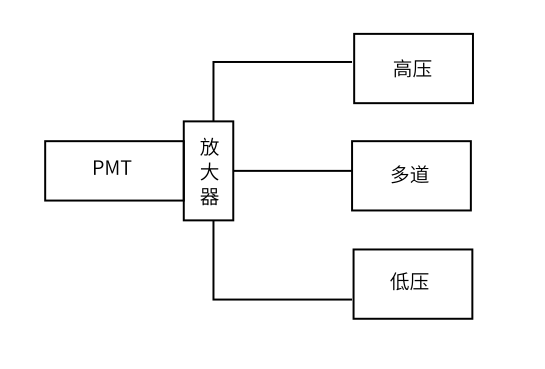
\includegraphics[width=0.45\textwidth]{yiqi.png}
\\
\xiaowu\song 图~1\begin{minipage}[t]{75mm} \quad 实验装置示意图。源发射的$\gamma$射线被光电倍增管接受后输入多道分析。\\[-1mm]\wuhao
\end{minipage}
\end{center}

首先打开仪器,调整高压和放大倍数到合适的范围。本实验中使用的高压为650V,放大倍数使得$^{60}$Co的全能峰在800道左右。

随后测量已知活度的$^{60}$Co,$^{137}$Cs,$^{54}$Mn能谱,并由此能谱标定能谱仪。测量和计算的相关信息如下表:

 \begin{center}
\bgliu
{\bf 表~1\quad
$^{60}$Co,$^{137}$Cs,$^{54}$Mn能谱以及活度数据表}\\[0.5mm]
\renewcommand{\arraystretch}{1.5}
\liuhao\song\rm
\newcolumntype{M}{>{\centering\arraybackslash}m{12mm} >{\centering\arraybackslash}m{14mm}
>{\centering\arraybackslash}m{12mm}>{\centering\arraybackslash}m{12mm}}
\begin{tabular}{M}
\specialrule{0.1em}{1pt}{1pt}

元素	&	能量/MeV	&	道址	&	活度/Bq	\\
\midrule
Co	&	1.17	&	689	&	8.23E+04	\\
-	&	1.33	&	785	&	-	\\
Cs	&	0.662	&	385	&	1.49E+05	\\
-	&	0.184	&	105	&	-	\\
Mn	&	0.835	&	488	&	2.02E+04	\\
\specialrule{0.1em}{3pt}{2pt}\\[-4mm]
\end{tabular}\\
\renewcommand{\arraystretch}{1.0}
\end{center}

可以作图拟合得到探测器系统道址和能量的对应关系,如下图所示:
\begin{center}
   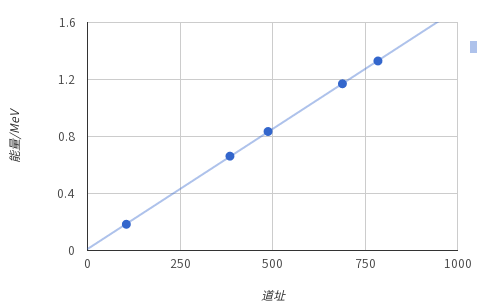
\includegraphics[width=0.45\textwidth]{1.png}
\\
\xiaowu\song 图~1\begin{minipage}[t]{75mm} \quad 谱仪道址和能量关系的标定图\\[-1mm]\wuhao
\end{minipage}
\end{center}
可以得到相应的现行关系,即:
\begin{equation}
   Energy = (1.684\times10^{-3} \times channel + 0.01)MeV
\end{equation}
以$^{60}$Co 1.33MeV能量的峰为标准可以得到探测器的能量分辨率为6.8\%。

\subsection{能谱分析}

首先是选取特征道。因为选取的原则是易于分辨,所以我们选择Co的1.33MeV, Cs的0.662MeV, Mn的0.835MeV三个峰作为特征峰位,相关的道址如下:

 \begin{center}
\bgliu
{\bf 表~2\quad
$^{60}$Co,$^{137}$Cs,$^{54}$Mn特征道域选取}\\[0.5mm]
\renewcommand{\arraystretch}{1.5}
\liuhao\song\rm
\newcolumntype{M}{>{\centering\arraybackslash}m{12mm} >{\centering\arraybackslash}m{12mm}
>{\centering\arraybackslash}m{12mm}}
\begin{tabular}{M}
\specialrule{0.1em}{1pt}{1pt}

元素	&	起始道址	&	终止道址	\\
\midrule
Co	&	755	&	815	\\
Cs	&	362	&	512	\\
Mn	&	464	&	408	\\
\specialrule{0.1em}{3pt}{2pt}\\[-4mm]
\end{tabular}\\
\renewcommand{\arraystretch}{1.0}
\end{center}

因而可以从能谱中得到在各个特征道域的计数。该计数应该减去本底计数。具体的数据如下表:

\begin{center}
\bgliu
{\bf 表~3\quad
$^{60}$Co,$^{137}$Cs,$^{54}$Mn以及混合样品在各个特征道域上的静计数。计数时间是1800s(等效活时间)。}\\[0.5mm]
\renewcommand{\arraystretch}{1.5}
\liuhao\song\rm
\newcolumntype{M}{>{\centering\arraybackslash}m{12mm} >{\centering\arraybackslash}m{12mm}
>{\centering\arraybackslash}m{12mm}>{\centering\arraybackslash}m{12mm}}
\begin{tabular}{M}
\specialrule{0.1em}{1pt}{1pt}
元素	&	Co道域计数	&	Cs道域计数	&	Mn道域计数	\\
\midrule
Co	&	1176676	&	777608	&	982837	\\
Cs	&	484	&	1622692	&	1908	\\
Mn	&	10190	&	43164	&	201623	\\
样品	&	791909	&	1721381	&	1120765	\\
\specialrule{0.1em}{3pt}{2pt}\\[-4mm]
\end{tabular}\\
\renewcommand{\arraystretch}{1.0}
\end{center}

用单位时间计数除以活度就可以得到对应的矩阵A。以及列向量M。 即

\begin{equation}
A = \begin{pmatrix}
7.94E-03 &
1.80E-06 &
2.80E-04 \\
5.25E-03 &
6.05E-03 &
1.19E-03 \\
6.63E-03 &
7.12E-06 &
5.55E-03 \\
\end{pmatrix}
\end{equation}
\begin{equation}
M=\begin{pmatrix}
4.40E+02	\\
9.56E+02	\\
6.23E+02
\end{pmatrix}
\end{equation}

根据逆矩阵即可解得对应的活度为
\begin{equation}
X=\begin{pmatrix}
5.3673\times 10^{4}\\
1.0210\times 10^{5}\\
4.7943\times 10^{4}
\end{pmatrix}
\end{equation}

即$^{137}$Cs、$^{60}$Co、$^{54}$Mn的活度分别为:$1.0210\times 10^{5}$Bq、$5.3673\times 10^{4}$Bq、$4.7943\times 10^{4}$Bq.

\section{误差分析}
根据误差理论推算出第j种成分含量$x_{i}$的标准误差:
\begin{equation}
\sigma _{x_{j} }=\frac{1}{\sqrt{t}}\sqrt{\sum_{j^{'}}^{3}\delta _{jj^{'}}x_{j^{'}}+B_{i}}
\end{equation}
其中:
\begin{equation}
\delta _{jj^{'}}=\sum_{i}^{3}(a_{ji}^{-1})^{2}a_{ij^{'}}
\end{equation}
表示第$j^{'}$成分计数的统计涨落对第j种成分的误差贡献因子。
\begin{equation}
B _{j}=2\sum_{i}^{3}(a_{ji}^{-1})^{2}b_{i}
\end{equation}

有
\begin{equation}
	(a_{ji}^{-1})^2 =\begin{pmatrix}
1.73E+04&	9.84E-04&	4.40E+01\\
6.93E+03&	2.73E+04&	9.73E+02\\
2.47E+04&	3.05E-02&	3.55E+04
\end{pmatrix}
\end{equation}

所以有
\begin{equation}
	\delta_{jj'} =\begin{pmatrix}
137.37&	90.877&	114.94\\
55.35&	202.70&	51.54\\
206.06&	171.92&	360.79
\end{pmatrix}
\end{equation}

\begin{equation}
	B=\begin{pmatrix}
	4246.3\\
	24888.7\\
	26010.4
	\end{pmatrix}
\end{equation}

标准误差为
\begin{equation}
	\sigma=\begin{pmatrix}
	4.71E+03\\
	5.14E+03\\
	6.78E+03
	\end{pmatrix}
\end{equation}

相对误差为Cs: 5.9\%, Co: 8.8\%, Mn:14.2\%。

\section{结论}

$^{137}$Cs、$^{60}$Co、$^{54}$Mn的活度分别为:$1.0210\times 10^{5}$Bq、$5.3673\times 10^{4}$Bq、$4.7943\times 10^{4}$Bq, 相对误差为Cs: 5.9\%, Co: 8.8\%, Mn:14.2\%。

\section{参考文献}

\noindent
[1] Peking Unviersity, Fudan University \ Nuclear Experment
\ Nuclear Publishing House, 1989 (in Chinese)

\noindent
 (北京大学,复旦大学.\ 原子核实验\ 原子能出版社,\ 1989)

\end{multicols}

\newpage


\section*{附录:思考题}
1、逆矩阵法解谱的条件是什么?这些条件在实验中应该如何保证?\\
条件见引言部分,实验中保证条件有测量时间基本一致,测量条件不变,以及样品中元素的选择比较合适。

2、特征道域选择一个既能表征能量的特征峰,又能区别其他核素的全能峰。道阈选的太宽会导致本底数目响应增大,造成误差
增大,道阈选的太窄,会导致道阈内计数率偏小,统计涨落因素对误差的影响增大。

\clearpage
%\end{CJK*}
\end{document}

